\documentclass{beamer}
\usepackage[utf8]{inputenc}
\usepackage[T1]{fontenc}
\usepackage{lmodern}
\usepackage[ngerman]{babel}
\usepackage{graphicx}
\usepackage{listings}
\usepackage{verbatim} % mainly for multi-line comments

\usetheme{Madrid}
\useinnertheme{rectangles}
\setbeamertemplate{navigation symbols}{}
\setbeamercovered{highly dynamic}

\title{Tracking juggling balls using the Kinect}
\author[Rolf $\cdot$ Thiemo $\cdot$ Flo]{Rolf Boomgaarden $\cdot$ Thiemo Gries $\cdot$ Florian Letsch}
\institute{Universität Hamburg}
\date{30. Mai 2013}

\begin{document}

\frame
{
\titlepage
}

\frame
{
\tableofcontents
}

\section{A Juggling Robot}

\begin{frame}{Let's go}

FIXME: Paper 

maybe abstract
   
\end{frame}

\begin{frame}{System description}
FIXME
\end{frame}

\begin{frame}{Image processing pipeline}
FIXME
\end{frame}


\section{Hough Transform}

\begin{frame}{Hough Transform}
\color{red}{   FIXME: Thiemo}
\begin{center}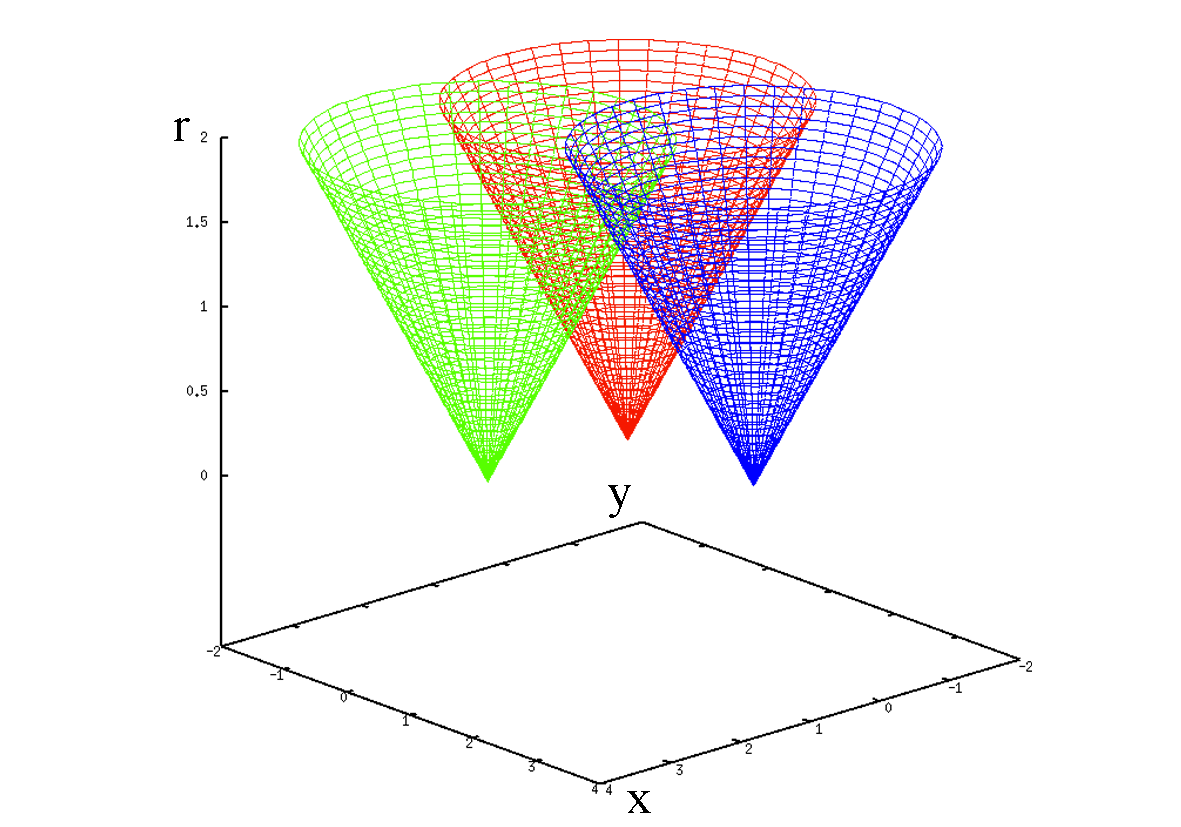
\includegraphics[0.5]{img/Hough3.png}\end{center}
\end{frame}

\section{Kalman Filter}

\begin{frame}
\frametitle{Kalman Filter}
\framesubtitle{sub}

FIXME: Rolf

\end{frame}

\begin{frame}{Conclusion}
   Video + paper conclusion
\end{frame}

\section{Our plan}
\begin{frame}{The flow}
IN: rgb + z

\begin{itemize}
	\item eliminate background in z
	\item search local maxima in z $\rightarrow$ ROIs
	\item use ROI mask on rgb
	\item Hough transform on rgb
	\item Match corresponding balls in multiple frames
	\item Kalman filter for each ball
\end{itemize}
\end{frame}

\begin{frame}{Challenges}
\begin{itemize}
	\item Local maxima
	\item Multiple balls (colour?)
\end{itemize}
\end{frame}

\begin{frame}{The end}
EOF
\end{frame}

\end{document}






